\chapter{Détection de groupes pertinents dans les flots de liens}
\minitoc
Nous avons vu précédemment qu'il était possible de trouver des groupes de liens dans un flots de liens via l'intermédiaire d'une projection du flot de liens en un graphe statique.
Parmi l'ensemble de ces groupes, il se peut que certains capturent des structures plus importantes et plus pertinentes que d'autres.
Le but ici est de réussir à extraire parmi ces groupes ceux qui sont pertinents.
En ce sens, nous nous posons la question de la décomposition partielle d'un flot de liens en sous-flots pertinents.
Il s'agit donc d'un problème légèrement différent de la détection de partition car certains liens peuvent n'appartenir à aucun groupe et les groupes doivent être pertinents.

Toute la difficulté pour réussir à trouver les groupes pertinents revient à trouver une définition convaincante de la pertinence.
La notion de densité est une première approche mais ce n'est pas suffisant.
En effet comme on a pu le voir précédemment, il peut exister de très grand groupes peu dense et de petits groupes très denses.
Faire la différence entre ces deux catégories en utilisant juste la densité n'est pas possible.
C'est pourquoi, nous utilisons une notion de voisinage.
Un groupe est alors pertinent si il est plus dense que son voisinage.
Ainsi, un groupe peu dense peut être pertinent si il est plus dense que son voisinage.
Comme le but est de pouvoir décrire le flot de liens, nous nous limitons aux groupes ayant une taille supérieur à un minimum.
Un exemple de flots avec une décomposition en groupes pertinent est dans la figure~\ref{fig:exemple_groupe_dens}.

Afin de trouver des des groupes pertinents, nous procédons de la manière suivantes:
\begin{itemize}
\item Nous construisons la projection du flot de liens en un graphe statique;
\item Nous appliquons sur cette projection un algorithme de détection de communautés afin d'obtenir une partition des liens du flot de liens;
\item Nous ne gardons dans la partition que les groupes qui sont considérés comme pertinent, c'est-à-dire ceux qui sont assez gros et qui sont plus dense que leur voisinage.
\end{itemize}

Afin de montrer la pertinence de cette approche, nous l'appliquons sur différents jeux de données et essayons de faire une analyse manuelle de certains groupes trouvés.
Par ailleurs, nous montrons que les groupes que nous détectons ne le sont pas par une méthode statique.

Le chapitre est organisé de la manière suivante.
Dans la section~\ref{sec:groupe_dense_existant}, nous revenons sur les travaux existants qui traitent de sujets similaire.
Puis dans la section~\ref{sec:groupe_dense_method}, nous présentons notre méthode de détection et de validation de groupes pertinents.
Enfin, les jeux de données que nous utilisons sont présentés dans la section~\ref{sec:groupe_dense_result} et les résultats associés dans la section~\ref{sec:groupe_dense_data}.

\begin{figure}
\centering
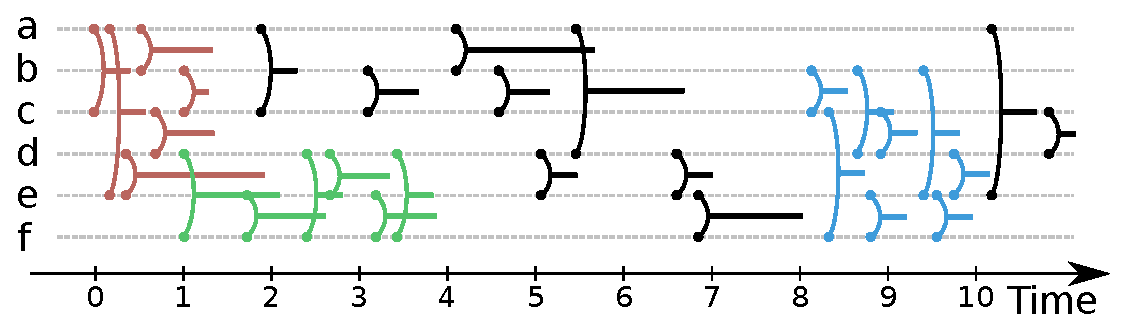
\includegraphics[width=\linewidth]{img/GroupeDense/GroupExample/Zone_dense.eps}
\caption{Exemple de flots de liens avec 3 groupes denses représenté par la couleur des liens (\textcolor{brique}{\textbf{rouge}}, \textcolor{vert_turquoise}{\textbf{vert}} et \textcolor{bleu_window}{\textbf{bleu}}).
}
\label{fig:exemple_groupe_dens}
\end{figure}

\section{Travaux existants}
\label{sec:groupe_dense_existant}


\section{\'Evaluation de la pertinence d'un groupe}
\label{sec:groupe_dense_method}

\section{Jeux de données}
\label{sec:groupe_dense_data}
\section{Application}
\label{sec:groupe_dense_result}



\section{Conclusion et perspective}


\subsection{Jeux de test ?}